\section{Implementation}

We structured our implementation in various components to keep the design modular and to lower complexity.
The main components of our design are the \textit{signal\_generator} unit, the \textit{moulator} unit and the
\textit{timekeeper} unit. These 3 components are wired together within the \textit{frequency\_modulation} unit.
An overview of the structure of our design can be seen in figure 2.

\begin{landscape}
	\begin{figure}[H] 
		%\centering % centering figure 
	    \scalebox{1.2} % rescale the figure by a factor of 0.8 
		{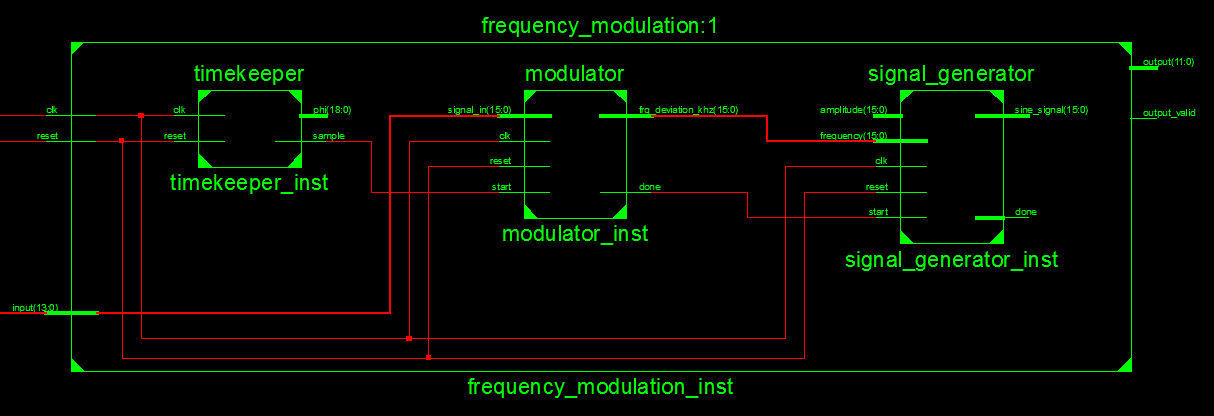
\includegraphics[height=6cm]{images/structure.png}} % importing figure
		\caption{Structural overview of the frequency\_modulation unit} 
		\label{fig:lorem} % labeling to refer it inside the text
	\end{figure} 
\end{landscape}

\subsection{timekeeper}

\begin{center}
	\begin{tabular}{ | l | c | l | }
		\hline
		\textbf{Generic} & \textbf{Default} & \textbf{Description} \\
		\hline
		DATA\_WIDTH & 8 & Defines the bit width of the signals in this entity \\
		CLK\_FREQ & 50000000 & Tells the component the clock speed the desing is running on \\
		BAUD\_RATE & 44000 & That many impulse signals per second will be generated \\
		\hline
	\end{tabular} 
\end{center}

\begin{center}
	\begin{tabular}{ | l | c | l | }
		\hline
		\textbf{Portname} & \textbf{Direction} & \textbf{Description} \\
		\hline
		clk & in & Clock signal \\
		reset & in  & Reset signal \\
		sample & out  & Impulse to be used as start flag for other components \\
		phi & out  & Values between $\pi$ and $-\pi$ to be used for testing \\
		\hline
	\end{tabular} 
\end{center}

The timekeeper unit correlates real time and clock time by generating \textit{BAUD\_RATE} impulses per second to be used as start signals for the other components. It also generates 
different continuos values between $\pi$ and $-\pi$ by incrementing an internal variable for the minimum precision $2^{DATA\_WIDTH}$ times per second. This can be used for testing.


\subsection{modulator}

\begin{center}
	\begin{tabular}{ | l | c | l | }
		\hline
		\textbf{Generic} & \textbf{Default} & \textbf{Description} \\ \hline
		DATA\_WIDTH & 8 & Defines the bit width of the signals in this entity \\
		MAX\_AMPLITUDE & 1.0 & Maximum expected amplitude of the input signal \\
		MIN\_AMPLITUDE & -1.0 & Minimum expected amplitude of the input signal \\
		FREQUENCY\_DEV\_KHZ & 0.5 & Maximum frequency deviation of the carrier rest frequency in kHz \\
		CARRIER\_FREQUENCY\_KHZ & 1.0 & Carrier rest frequency in kHz \\
		\hline
	\end{tabular} 
\end{center}

\begin{center}
	\begin{tabular}{ | l | c | l | }
		\hline
		\textbf{Portname} & \textbf{Direction} & \textbf{Description} \\
		\hline
		clk & in & Clock signal \\
		reset & in  & Reset signal \\
		start & in  & Start flag signals the component that it should start calculations \\
		done & out  & Done bit signals that calculations have been completed and the output is holding valid data \\
		signal\_in & in  & Sample value of the modulation signal \\
		frq\_deviation\_khz & out  & Calculated frequency to be used as input for the signal generator \\
		\hline
	\end{tabular} 
\end{center}

The modulator takes sample values of the modulation signal and translates them into a frequency. According to \textit{MIN\_AMPLITUDE} and \textit{MAX\_AMPLITUDE} it calculates a mean voltage level. A deviation from this voltage level translates to an increase or decrease of \textit{frq\_deviation\_khz}. Negative deviation of the mean amplitude correlates to a decrease of \textit{frq\_deviation\_khz} and positive deviation results in an increase. If there is no deviation at all the output shows the rest frequency of the carrier provided by the generic \textit{CARRIER\_FREQUENCY\_KHZ}.

\subsection{signal generator}

\begin{center}
	\begin{tabular}{ | l | c | l | }
		\hline
		\textbf{Generic} & \textbf{Default} & \textbf{Description} \\ \hline
		DATA\_WIDTH & 8 & Defines the bit width of the signals in this entity \\
		BAUD\_RATE & 44000.0 & The baudrate of the signal generator \\
		\hline
	\end{tabular} 
\end{center}

\begin{center}
	\begin{tabular}{ | l | c | l | }
		\hline
		\textbf{Portname} & \textbf{Direction} & \textbf{Description} \\
		\hline
		clk & in & Clock signal \\
		reset & in  & Reset signal \\
		start & in  & Start flag signals the component that it should start calculations \\
		done & out  & Done bit signals that calculations have been completed and the output is holding valid data \\
		frequency & in  & The frequency of the generated sign signal \\
		amplitude & in  & The amplitde of the generated sign signal \\
		sine\_signal & out  & The current sample of the generated sign signal \\
		\hline
	\end{tabular} 
\end{center}

The \textit{signal\_generator} is the core component of the design. The component instantiates the \textit{sine\_cordic} component we developed for the first task to generate a continuous set of sine wave samples with frequency and amplitude according to its inputs. 


\subsection{frequency modulation}

\begin{center}
	\begin{tabular}{ | l | c | l | }
		\hline
		\textbf{Generic} & \textbf{Default} & \textbf{Description} \\ \hline
		INTERNAL\_DATA\_WIDTH & 16 & Defines the bit width of the signals in this entity \\
		INPUT\_DATA\_WIDTH & 14 & Data width of the ADC register \\
		TIME\_PRECISION & 19 & Time precision data width to be used in the \textit{timekeeper} \\
		OUTPUT\_DATA\_WIDTH & 12 & Data width of the DAC register \\
		CLK\_FREQ & 50000000 & The clock frequency of the design \\
		BAUD\_RATE & 44000.0 & The baudrate of the signal generator \\
		CARRIER\_FREQ & 1.0 & Maximum frequency deviation of the carrier rest frequency in kHz \\
		FREQUENCY\_DEV\_KHZ & 0.5 & Maximum frequency deviation of the carrier rest frequency in kHz \\
		\hline
	\end{tabular} 
\end{center}

\begin{center}
	\begin{tabular}{ | l | c | l | }
		\hline
		\textbf{Portname} & \textbf{Direction} & \textbf{Description} \\
		\hline
		clk & in & Clock signal \\
		reset & in  & Reset signal \\
		input & in  & Sample of the ADC \\
		output\_valid & out  & Valid data flag to be written to the DAC \\
		output & out  & Output value to be written in the DAC register \\
		\hline
	\end{tabular} 
\end{center}

The frequency modulation component is wiring all the component together. It connects the sample impulse signals of the \textit{timekeeper} to the input \textit{start} ports of the other components. It wires the \textit{input} port to the \textit{signal\_in} port of the modulator, the \textit{frq\_deviation\_khz} output port of the \textit{modulator} to the \textit{frequency} input port of the \textit{signal\_generator} and the \textit{sine\_signal} output port of the \textit{signal\_generator} to the \textit{output} port of the \textit{frequency\_modulator}.




